%% ============================================================================
%% ============================================================================
\begin{frame}
\frametitle{Subproduct tree representation in CUDA}

\begin{itemize}
\item A subproduct tree on $n = 2^k$ points consists
      of $k$ levels (not counting the root).  
\item At level $h = 0$ (the leaves)
      we have $2^k$ polynomials of degree $2^0$, amounting to 
       $2^k (2^0 + 1)$ coefficients in total.
\item At level $h$, we have $2^{k-h}$ polynomials of degree $2^h$, amounting to 
       $2^{k-h} (2^h + 1)$ coefficients in total.
\item The total number of coefficients is
\begin{equation*}
2^{k+1} + k 2^k -2
\end{equation*}
\item Assuming that each coefficient requires 4 bytes and that
our GPU has 3 Giga-bytes of global memory, the largest possible $k$ is $24$.
\item In the GPU global memory, the subproduct tree is an array
      storing successively the polynomials at lelvel $h=0$, $h=1$,
     \ldots $h = k -1$.
\end{itemize}
\end{frame}
%% ============================================================================
%% ============================================================================
\begin{frame}
\frametitle{Polynomial multiplication in CUDA}
\begin{itemize}
\item We rely on FFT-based multiplication in input degree higher than $2^8$.
      (M.M.M. \& Wei Pan, Journal of Physics Conference Series, 2011).
\item In lower degree, we rely in plain quadratic multiplication.
\item The table below compares our FFT-based multiplication and an
      optimized plain multiplication for 
       $(t, w) \in \{ (128, 4), (128, 8),  (256, 4), (256, 8) \}$
      where $t$ is the numberof threads per block and $w$
       the number of coefficients per thread.
\end{itemize}

\begin{tabular}{ l || l | l | l | l | l |l |}
\hline
Length & FFT-based & Opt 1 & Opt 2 & Opt3 & Opt4 \\
\hline
8 & 4.168448 & 0.147488 & 0.138048 & 0.151136 & 0.140608 \\
9 & 3.866848 & 0.230976 & 0.157984 & 0.215872 & 0.159136 \\
10 & 5.014496 & 0.513888 & 0.334464 & 0.496096 & 0.305600 \\
11 & 5.299264 & 1.667808 & 0.870688 & 1.875936 & 0.964352 \\
12 & 5.944992 & 6.31552 & 3.115360 & 7.439104 & 3.572864 \\
13 & 6.267520 & 25.045984 & 12.077248 & 29.626495 & 14.270720\\
14 & 7.050112 & 20.753984 & 47.733665 & 64.931938 & 57.355328\\
\hline
\end{tabular}

\end{frame}

%% ============================================================================
%% ============================================================================
\begin{frame}
\frametitle{Subproduct tree construction in CUDA (1/3)}

\begin{itemize}
\item The subproduct tree is built bottom-up, starting from the leaves.
\item Building level $h+1$ from level $h$ is done by a series of CUDA kernel calls.
\item Each level from $h=0$ to $h=7$ involves multiplication in degree $2^7$ or less,
      thus it is performed by a \blue{list of plain multiplications}.
\item Each of the higher levels requires FFT-based multiplication, thus
        \blue{list of direct FFTs}, followed by 
         \blue{list of pointwise multiplications}, followed by 
      \blue{list of inverse FFTs}.
\end{itemize}
\end{frame}
%% ============================================================================
%% ============================================================================
\begin{frame}[shrink=20]
\frametitle{Subproduct tree construction in CUDA (2/3)}
\begin{tabular}{l || l | l}
Input Size (${\log}_2$ of) & Time (ms) & Memory (Bytes)\\
\hline
%% 3 & 0.057280 & 56\\
4 & 0.070720 & 152\\
5 & 0.111808 & 376\\
6 & 0.323840 & 888\\
7 & 0.468992 & 2040\\
8 & 0.829888 & 4600\\
9 & 1.995616 & 10232\\
10 & 5.477760 & 22520\\
11 & 8.468224 & 49144\\
12 & 12.787584 & 106488\\
13 & 15.839264 & 229368\\
14 & 24.897984 & 491512\\
15 & 35.802338 & 1048568\\
16 & 56.436737 & 2228216\\
17 & 89.414787 & 4718584\\
18 & 161.420929 & 9961464\\
19 & 298.262054 & 20971512\\
20 & 587.439819 & 44040184\\
21 & 1180.089966 & 92274680\\
22 & 2308.174072 & 192937976\\
23 & 4549.854980 & 402653176\\
24 & 8180.691895 & 838860792\\
\end{tabular}
\end{frame}
%% ============================================================================
%% ============================================================================
\begin{frame}
\frametitle{Subproduct tree construction in CUDA (3/3)}
\begin{center}
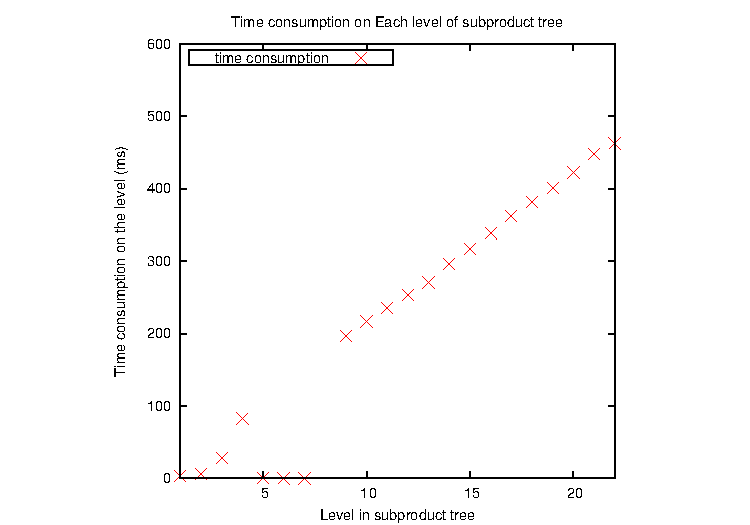
\includegraphics[scale=0.9]{images/sub_product_tree_step.pdf}
\end{center}
\end{frame}
%% ============================================================================
%% ============================================================================
\begin{frame}
\frametitle{Fast multi-point evaluation in CUDA (1/3)}
\begin{itemize}
\item The fast multi-point evaluation proceeds in a top-down manner.
\item Moving from lelvel $h$ down to level $h-1$ is done by a series of CUDA kernel calls.
\item Each level from $h=0$ to $h=7$ involves plain division.
\item Each of the higher levels uses \blue{fast division}.
\item The \blue{power series inversion} uses plain (quadratic) multiplications in low
      degree and FFT-based multiplication from degree $2^8$.
\end{itemize}
\end{frame}
%% ============================================================================
%% ============================================================================
\begin{frame}[shrink=20]
\frametitle{Fast multi-point evaluation in CUDA (2/3)}
\begin{tabular}{ l | l }
Input size  (${\log}_2$ of)  & Time (ms) \\
\hline
% 2 & 0.066016 \\
% 3 & 0.039424 \\
4 & 0.064032 \\
5 & 0.102784 \\
6 & 0.176448 \\
7 & 0.320640 \\
8 & 0.627616 \\
9 & 1.181408 \\
10 & 2.019488 \\
11 & 53.894718 \\
12 & 113.643204 \\
13 & 178.820190 \\
14 & 261.687347 \\
15 & 360.460541 \\
16 & 511.921570 \\
17 & 791.367065 \\
18 & 1216.930176 \\
19 & 2084.443359 \\
20 & 3773.393066 \\
21 & 7177.844238 \\
22 & 14181.632812 \\
23 & 28927.501953 \\
\end{tabular}
\end{frame}
%% ============================================================================
%% ============================================================================
\begin{frame}
\frametitle{Fast multi-point evaluation in CUDA (3/3)}
\begin{center}
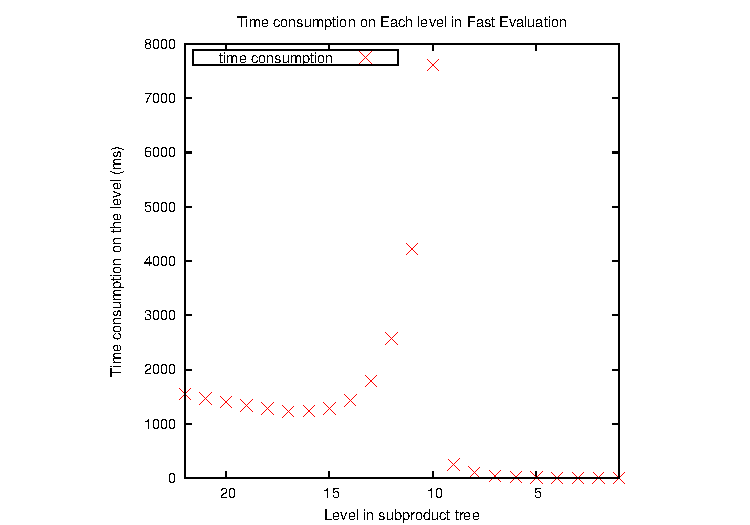
\includegraphics[scale=0.9]{images/fast_evaluation_step.pdf}
\end{center}
\end{frame}
%% ============================================================================
%% ============================================================================
\begin{frame}
\frametitle{Conclusions}

\end{frame}
%% ============================================================================
